\documentclass{article}
\usepackage[utf8]{inputenc}

\title{CS685 Data Mining - Assignment2}
\author{P J Leo Evenss(20111038) }
\date{\today}
\usepackage{graphicx}
\usepackage[section]{placeins}
\usepackage{hyperref}
\hypersetup{
    colorlinks=true,
    linkcolor=blue,
    filecolor=magenta,      
    urlcolor=cyan,
}

\urlstyle{same}
\begin{document}



\maketitle

\section{Introduction}
\vspace{0.5cm} 
\hspace{2cm} This assignment enlightens us with the basic knowledge of graph mining, and helps us to understand better how the websites are interlinked and maintained in the internet. The tasks given to solve, helps us in getting a short insight of how the articles and categories are grouped in the  game of Wikispeedia which collects the navigation of humans in the Wikipedia articles. The game focuses on Semantic Distance Measure among the articles found in internet.

\section{Analysis}
\vspace{0.5cm} 
\hspace{2cm}The overview analysis of the assignment is done as below:
\subsection{Article Categories}
\vspace{0.5cm} 
\hspace{2cm}
All the articles are placed in the respective 146 Categories, so as to maintain a well-defined dataset and the mapping of articles to categories is done.  
\subsection{Article Graph}
\vspace{0.5cm} 
\hspace{2cm}
The articles in the wikispeedia dataset is stored in the form of directed graphs, the Figure 1 shows the number of components and the nodes and edges present for the respective component.  
\begin{figure}[htp]
    \centering
    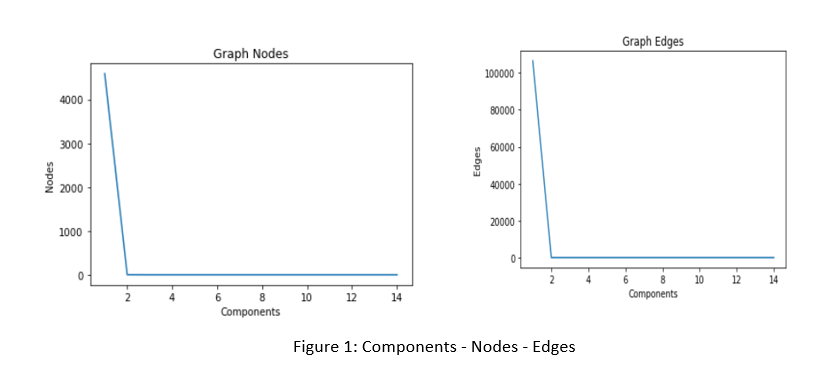
\includegraphics[width=12cm]{graphs.png}
    \caption{The graph of connected components and its nodes and edges}
    \label{fig:graphs}
\end{figure}
\FloatBarrier
 
\hspace{2cm}
We can observe that the 99\% of the articles are connected in a single component, while other components have isolated edges. 
The undirected graph is taken into consideration for approximation in the assignment.
\subsection{Article Paths}
\vspace{0.5cm} 
\hspace{2cm}
The paths taken for reaching the destination from the source are provided and the analysis is done for finding the length of the path the human took and its corresponding shortest path. 
The percentage ratios of human path vs shortest path is plotted considering the back clicks and also without back clicks in the below Figure 2

\begin{figure}[htp]
    \centering
    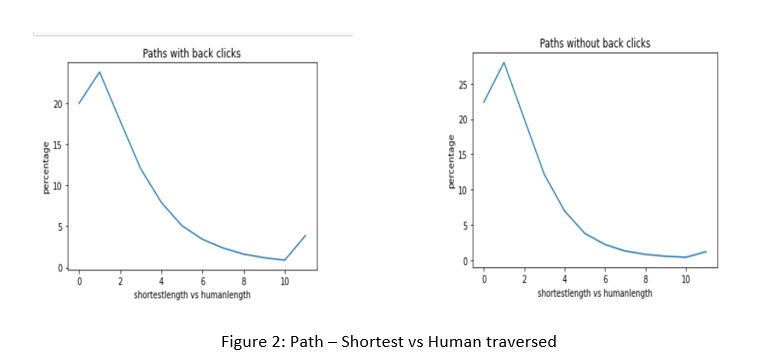
\includegraphics[width=12cm]{hp-sp.png}
    \caption{The percentage of human vs shortest path}
    \label{fig:graphs}
\end{figure}
\FloatBarrier
We observe that 19\%-23\% of the paths have equal human length and shortest path length with and without back clicks respectively, inferring that these paths have been correctly traversed with minimum number of article visits.

\subsection{Path Categories}
\vspace{0.5cm} 
\hspace{2cm}
The below Figure 3 shows the distribution of the categories visited in each path.
\begin{figure}[htp]
    \centering
    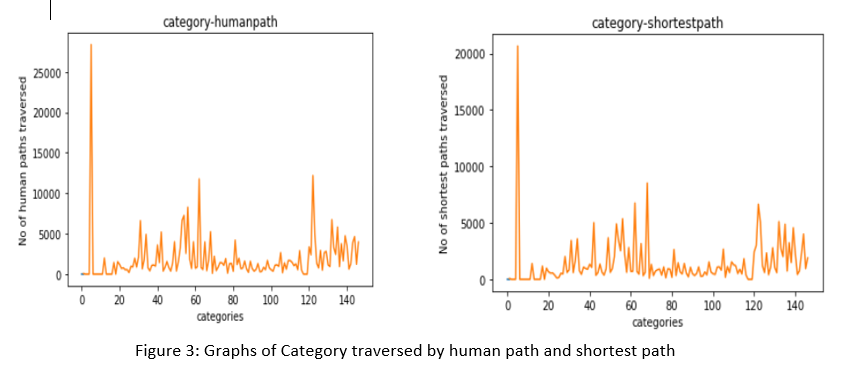
\includegraphics[width=12cm]{cat-path.png}
    \caption{The Categories visited in human path and shortest path}
    \label{fig:graphs}
\end{figure}
\FloatBarrier
 
\hspace{2cm}
We can infer the number of paths that enclosed each category, while traversing by the human as well as in the shortest path of the graph. \subsection{Category Pairs}
\vspace{0.5cm} 
\hspace{2cm}
The Category pairs of source and destination of the finished and unfinished paths are evaluated. These results gives us a view of the mapping of categories with each other and the number of paths that had articles traversing from one category to another, Eventually creating a graph of categories with edges from source to destination category. 
\subsection{Category Ratios}
\vspace{0.5cm} 
\hspace{2cm}
The Category pairs are being considered as nodes and edges of the graph. The paths these category pairs fall in and the length of human path and shortest path and their respective ratios are calculated. The shortest path indicates the shortest distance between the category 1 and category 2 in the category pairs and the ratio  indicates the average number of extra articles traversed by the human than the shortest path to reach the destination category.
\section{Conclusion}
\vspace{0.5cm} 
\hspace{2cm}
Thus we did a small part in learning and analysing the storage of articles in graph based structures in the Wikipedia and the respective dataset collected through the Wikispeedia game.


\end{document}
